\question 下面有关选择进程调度算法的准则中不正确的是
\par\fourch{为了尽快响应交互式用户的请求,可以采用时间片轮转调度策略}{为了尽量提高处理器利用率,可以适当提高I/O型作业的并发程度}{为了尽可能降低作业周转时间,可以采用动态优先级调度策略}{\textcolor{red}{为了尽可能提高吞吐量,可以优先执行短作业}}
\begin{solution}调度算法要达到的目的主要有以下4点:尽量加快响应速度,尽量提高处理器利用率,尽量提高系统吞吐量,尽量降低作业周转时间。关键词:响应速度、CPU利用率、系统吞吐量、作业周转时间。
为了尽量及时地响应每个用户的请求,通常系统会采用时间片轮转调度策略,这样可以在相对短的时间内,对每个用户的请求都做出响应,A选项正确。
I/O型作业的特点是CPU使用的比例不大,大部分时间在进行I/O操作,CPU比较空闲,因此可以适当提高这类作业的并发度,提高CPU的利用率,B选项正确。
在采用了优先级的系统中,有些优先级低的作业会由于总有优先级高的作业到达而长期得不到执行,导致周转时间过长,为了解决这种情况,引入动态优先级的概念,随着等待时间变长,作业的优先级逐渐提高,这样每个作业的周转时间都不会太长。采用动态优先级可以降低那些低优先级作业的周转时间,C选项正确。
在短作业较多的系统中,由于执行每个作业的时间较短,因此系统的吞吐量会比较大。虽然优先执行短作业会提高系统吞吐量,但是如果只考虑优先执行短作业的话,则会使长作业长期得不到调度,导致这些作业``饿死'',并不可取。因此D选项错误。
\end{solution}
\question (西安电子科技大学,2000年)设有4个作业同时到达,每个作业的执行时间均为2小时,它们在一台处理机上按单道方式运行,则平均周转时间是(
)小时
\par\twoch{1}{\textcolor{red}{5}}{2.5}{8}
\begin{solution}从进程提交到进程完成的时间间隔为周转时间,即周转时间=等待时间+运行时间。按执行顺序,4个作业的周转时间分别为2、4、6、8个小时。平均周转时间=(2+4+6+8)/4=5(小时)。
\end{solution}
\question 某系统正在执行三个进程P1、P2和P3,各进程的计算(CPU)时间和I/O时间比例如下表所示。为提高系统资源利用率,合理的进程优先级设置应为(
~)。
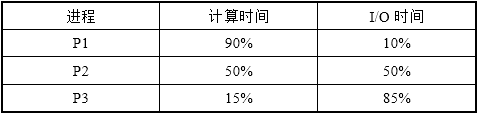
\includegraphics[width=3.33333in,height=0.79167in]{computerassets/DF32FF3C08A6FE076B80C8533203918A.png}
\par\fourch{}{\textcolor{red}{}}{}{}
\begin{solution}首先要知道一个前提,进程多数都是先计算后I/O的(先I/O后计算的任务无意义),所以常常空闲的是I/O设备,因此提高I/O的利用率,就能提高整个系统的资源利用率。这里设置的进程优先级越高,那么CPU就会优先进行处理,因此要想提高CPU和I/O设备的并行性,就需要让I/O繁忙型的进程优先由CPU进行处理,减少其等待时间,也就减少了I/O设备的空闲时间。因此,优先级最高应选择I/O时间占最大的P3,次之P2,最后P1。
~ ~ ~ ~~

注意:其实本题考查的就是短进程优先调度算法,原理是一样的。
\end{solution}
\question 操作系统的( )管理部分负责对进程进行调度
\par\twoch{主存储器}{控制器}{运算器}{\textcolor{red}{处理机}}
\begin{solution}对第二章有所了解就会知道,进程管理就是控制进程如何使用处理机(计算机系统中最宝贵的资源),所以归类于处理机管理部分。
依照这种思路,还可以考查其他资源管理,比如请求分页属于存储器管理部分,目录结构属于文件管理部分等。这里有个技巧,在复习操作系统的时候应该会发现,操作系统的章节是按照四种资源的管理分类安排的,从进程管理开始每章都是对于一种资源的管理,因此只要知道考查的是哪一章的内容就可以知道是属于哪种资源管理部分了。这也是复习操作系统的一个整体框架。
以上三道题都是对操作系统功能和概念的典型考查,一般题目都大同小异,无非是考查操作系统是什么,功能是什么。只要记住这些,操作系统概念的题目也就拿下了。
\end{solution}
